\documentclass[]{article}

\usepackage{graphicx}   
\usepackage[utf8]{inputenc}
\usepackage{listings}
\usepackage{hyperref}
\usepackage{tabularx}
\usepackage{subfig}
\usepackage{float}
\usepackage{graphicx}
\usepackage{subfig}
\graphicspath{ {imagenes/} }
\usepackage{xcolor}
\definecolor{RoyalBlue}{cmyk}{1, 0.50, 0, 0}
\usepackage{listings}
\lstset{language=Java,
	keywordstyle=\color{RoyalBlue},
	basicstyle=\scriptsize\ttfamily,
	commentstyle=\ttfamily\itshape\color{gray},
	stringstyle=\ttfamily,
	showstringspaces=false,
	breaklines=true,
	frameround=ffff,
	frame=single,
	rulecolor=\color{black}}



%opening
\title{Práctica 4 SS}
\author{José Manuel Pérez Lendínez, 26051613-l}

\begin{document}
\newcolumntype{M}{>{\begin{varwidth}{4cm}}l<{\end{varwidth}}}	
	\maketitle
	
	
	\newpage
	\tableofcontents
	\newpage

\section{Expiación del trabajo a realizar}
En este caso vamos a crear un sistema para simular el modelo o de ecosistema Lotka-Volterra. Se define con el siguiente sistema de ecuaciones diferenciales:
$$\frac{d x}{d t}=a_{11} x-a_{12} x y$$
$$\frac{d y}{d t}=a_{21} x y-a_{22} y$$
En nuestro caso x serán las presas (conejos) e y serán los depredadores (zorros). Cada una de las especies tienen unas características que indicaran como evolucionan la población. Estas características nos indicarán los siguiente:
\begin{enumerate}
	\item \textbf{$a_{11}$:} Tasa de crecimiento de los conejos. Por cada individuo tendremos $a_{11}$ descendientes.
	\item \textbf{$a_{12}$:} Indica la cantidad de conejos que es capaz de capturar un zorro de media.
	\item \textbf{$a_{21}$:} Indica la importancia de la comida para conseguir sobrevivir los zorros.
	\item \textbf{$a_{22}$:} En este caso marcara el numero de individuos que mueren de los zorro. 
\end{enumerate}

Una vez explicado esto vamos a explicar la forma de llamar a nuestro programa:
$$ ./simulador\ a11\ a12\ a21\ a22\ Tinicio\ Tfin\ Poblacionx\ Poblaciony\ dt\ Tipo$$

Vamos a explicar los parámetros:
\begin{enumerate}
	\item \textbf{$a_{11}\ a_{12}\ a_{21}\ a_{22}$:} Esto corresponde a las características explicadas anteriormente.
	\item \textbf{Tinicios:} Indica el tiempo en el que se iniciaría la simulación.
	\item \textbf{Tfin:} Sera el tiempo en el que el simulador dejara de ejecutar al alcanzarlo.
	\item \textbf{Poblacionx:} Numero de conejos iniciales al empezar la simulación.
	\item \textbf{Poblaciony:} Numero de zorros iniciales al empezar la simulación.
	\item \textbf{Dt:} Indica el tiempo que avanzaremos en cada ciclo del simulador.
	\item \textbf{Tipo:} Lo utilizamos para elegir entre euler y runge-kutta, de forma que si se introduce un 1 se cambiara a runge-kutta y en caso de introducir otro valor se usara euler. 
\end{enumerate}

Con esto ya tenemos todo lo necesario para entender el simulador y poder iniciar las pruebas de su funcionamiento
\newpage
\section{Pruebas del simulador}
\subsection{Valores iniciales}
Empezaremos por una simulación inicial en la que tendremos tendremos los datos dados en la practica para iniciar. Dichos datos son los siguientes: 
$$a_{11}=5\ a_{12}=0.05\ a_{21}=0.0004\ a_{22}=0.2$$

Para ver la evolución de la población mostraremos una grafica donde se vera como va evolucionando la población con el tiempo transcurrido. En este caso tendremos un tiempo de inicio de 0 y un tiempo de fin de 300. Las poblaciones inicial serán también las dadas en las diapositivas, 500 conejos y 100 zorros. El parámetro dt coincide con el 0.1 especificado en el pdf de la practica y utilizaremos runge-kutta. Utilizare estos valores por defecto en las siguientes ejecuciones si no se especifica algún cambio.

Vamos a mostrar la grafica de evolución para poblaciones para estos parámetros:
\begin{figure}[H]
	\centering
	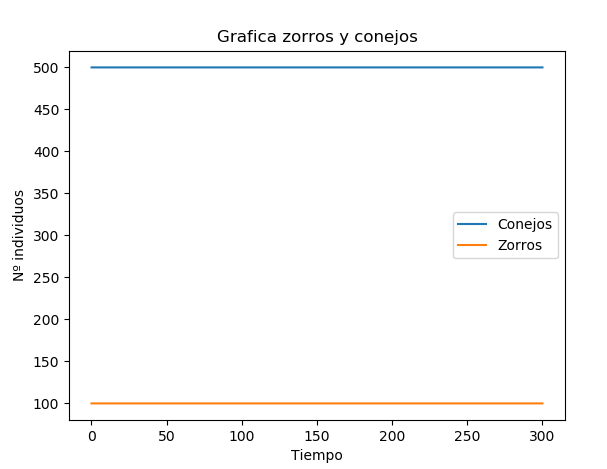
\includegraphics[width=1\linewidth]{screenshot001}
\end{figure}

Como se ve en la grafica con estos valores tenemos una población estable que no varia en ningún momentos de la cantidad inicial de individuos. Esto nos indica que los parámetros equilibran la población y a partir de estos podremos cambiarlos para ver como varían y como afecta realmente a  la población. Con esto también podemos ver que ahora mismo los parámetros están especificados de una manera en la que para que cambie alguna de las dos poblaciones tiene que cambiar la población contraria. De forma que el numero de zorros depende del numero de conejos y al contrario.

\subsection{Cambios en las población unicamente.}
\subsubsection{Subida en la poblacion de zorros}
Vamos a realizar un cambio en la población inicial de zorros para ver esto como afecta la sistema.
Para esto cambiaremos el parámetro Poblaciony, dándole un valor de 200. 
\begin{figure}[H]
	\centering
	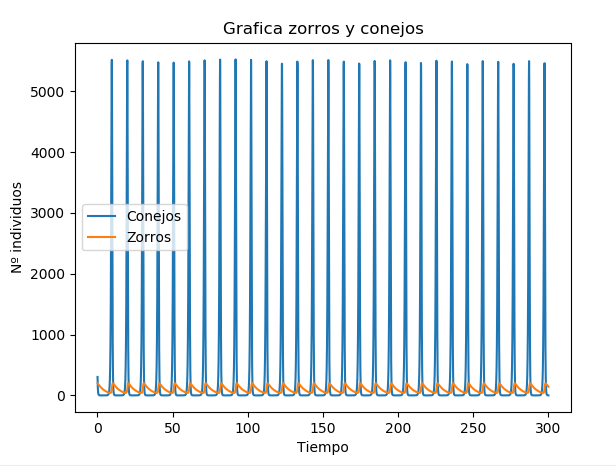
\includegraphics[width=1\linewidth]{screenshot002}
\end{figure}
En este caso vemos claramente dos cosas importantes que nos mostrara como afecta el numero de una población a la otra. En el momento en el que empieza a crecer la población de conejos, la poblacion de zorros sube también al mismo tiempo. Pero esto lleva a un punto en el que se alcanza el máximo de conejos y zorros que podremos tener a la misma vez. Una vez alcanzado este momento se ve claramente como la poblacion de conejos baja de golpe muy bruscamente hasta valores cercanos de 0 y se mantiene en esos niveles mientras la población de zorros decrece de una forma mas lenta. En el momento en el que la población de zorros llega también a valores cercanos a 0, vemos como la población de conejos sube rápidamente y llega nuevamente a su punto máximo, subiendo a la misma vez la población de zorros nuevamente a su punto máximo.
\newline

Vamos a ver la grafica donde mostramos los valores de una poblacion frente la otra para ver si coincide con lo que hemos obtenido hasta este momento.
\begin{figure}[H]
	\centering
	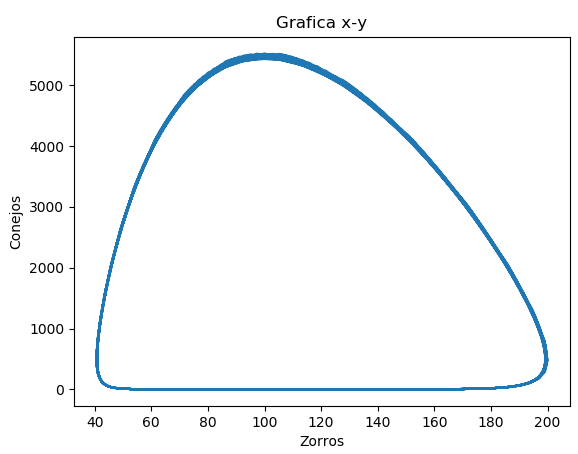
\includegraphics[width=1\linewidth]{screenshot004}
\end{figure}


Esta grafica nos muestra lo dicho anteriormente. Se ve claramente el ciclo en el que llegado un momento ambas especies están al borde de la extinción con la linea cerca del 0.  Llegado ese momento vemos como sube mucha la población a su máximo y vuelve a bajar de nuevo de forma muy brusca en ambos caso. También podemos ver como la subida que corresponde a la parte derecha izquierda de la grafica es algo mas brusca que la bajada que corresponde a la parte derecha. Esto se da porque en la subida tanto los zorros como los conejos crecen muy rápido, en cambio en la bajada se ve como aunque los conejos si bajan muy rápido, la bajada de la población de zorros se prolonga mas en el tiempo.
\newpage
\subsubsection{Subida en la población de conejos}
En este caso la población de zorros volverá a ser de 100 y subiremos la población de conejos a 600 para ver como afecta en este caso. Para esto el parámetro poblaciony sera 100 y poblacionx sera de 600.
Vamos a mostrar la grafica con ambas poblaciones por separado.
\begin{figure}[H]
	\centering
	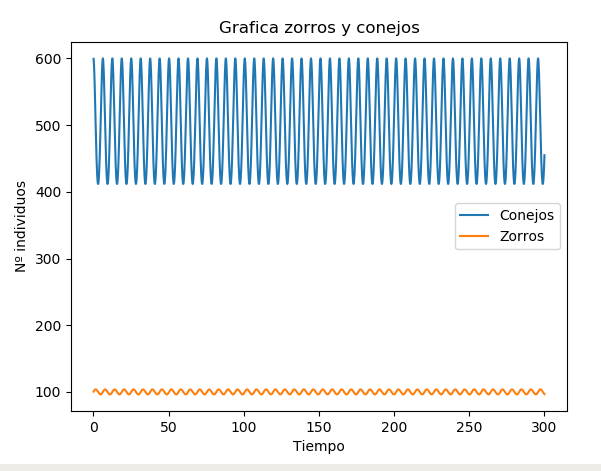
\includegraphics[width=1\linewidth]{screenshot005}
	\caption{}
	\label{fig:screenshot005}
\end{figure}
En este caso se ven unos cambios menos bruscos que anteriormente y mas estables. Se dan también momentos en los que tenemos un mayor numero de zorros y conejos pero dichos pero no están tan cerca de la extinción como en el caso anterior. Al tener una población mas controlada, se ve como cuando se llega a la población máxima de conejos la poblacion de zorros estaba en su punto mas bajo, y como esta empieza a remontar y la de conejos empieza a bajar hasta llegar los conejos a su nivel mas bajo de población. Una vez llegado a su numero mas bajo los conejos los zorros empiezan a bajar su población y los conejos aumentan la suya hasta que los zorros llegan a su nivel mas bajo nuevamente y los conejos a su nivel mas alto. 
\newpage

Vamos a ver si esto coincide con el grafico que nos muestra los valores de ambas poblaciones enfrentados.

\begin{figure}[H]
	\centering
	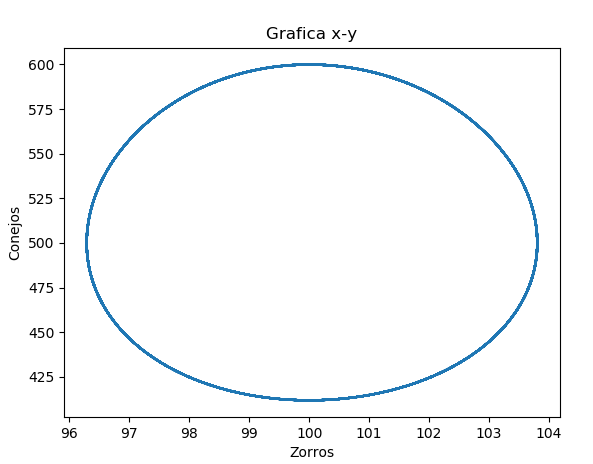
\includegraphics[width=1\linewidth]{screenshot006}

\end{figure}
En esta grafica se muestra lo explicado anteriormente. Sabemos que se da esto puesto que se da un circulo sin tener ninguno de los dos lazos del circulo un cambio mas brusco como en el caso anterior. Con esto se ve claramente que este modelo es mas sostenible que el anterior y no esta tan cerca de la extinción como el anterior.
\newpage
\subsection{Cambios en $a_{ij}$.}
En este caso vamos a dejar las poblaciones con los valores iniciales de 500 y 100, cambiando los valores $a_{ij}$ para ver como afectan estos a la población realmente. Cambiaremos los parámetros de uno en uno dejando los demás con los valores iniciales.
\subsubsection{Mejoramos la eficiencia en la caza.}
En este caso cambiaremos el parámetro $a_{12}$ para ver como afecta la mejora en la caza. Le vamos a dar un valor de 0.1 en vez de los 0.05 anteriores. Mostramos las graficas y a continuación las explicamos.


\begin{figure}[H]
	\centering
	\subfloat{
		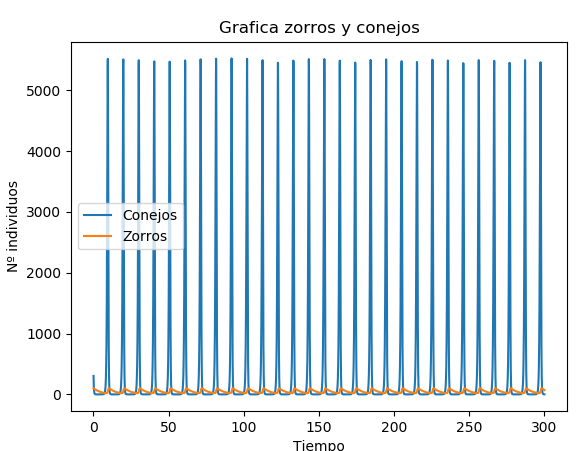
\includegraphics[width=0.5\textwidth]{screenshot007}}
	\subfloat{
		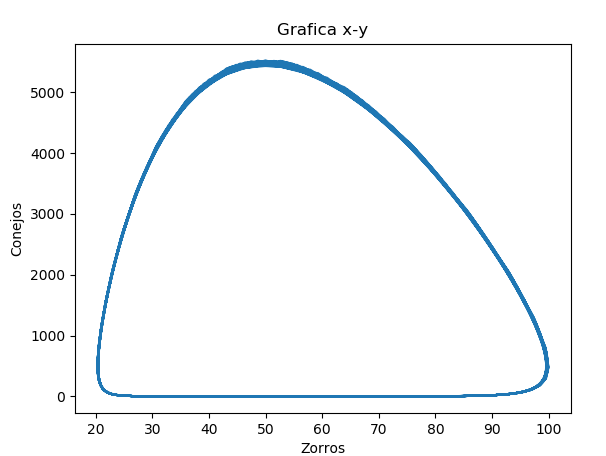
\includegraphics[width=0.5\textwidth]{screenshot008}}

\end{figure}

En este caso se ve algo parecido al caso en el que se aumento la población de zorros, esto es debido a que al aumentar las capacidades de cazas de los zorros, estos consiguen un mayor numero de presas que antes. Al cazar mas que antes las presas bajan rápidamente y no queda alimento para los zorros y estos empiezan a bajar nuevamente la poblacion y suben los conejos. Esto se repite continuamente como en caso anterior. La diferencia con el caso nombrado es que la poblacion de zorros no tiene una subida tan fuerte como en ese caso siendo un poco mas suave. 
\newpage
\subsubsection{Mejoramos la natalidad de las presas}
Vamos a aumentar el parámetro $a_{11}$ de forma que en vez de 5 criás por presa aumentaremos a un total de 10. A continuación mostrare las graficas y las analizaremos

\begin{figure}[H]
	\centering
	\subfloat{
		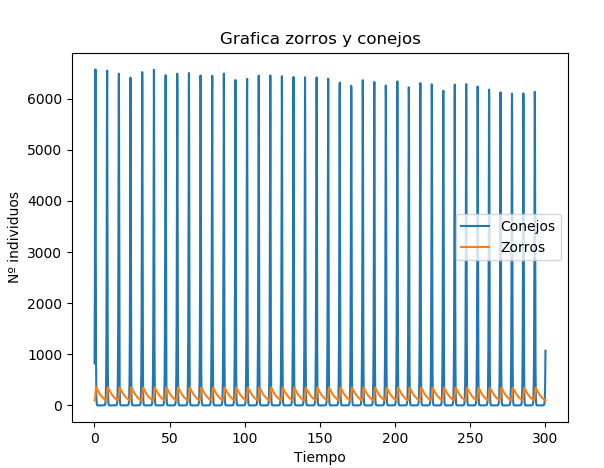
\includegraphics[width=0.5\textwidth]{screenshot010}}
	\subfloat{
		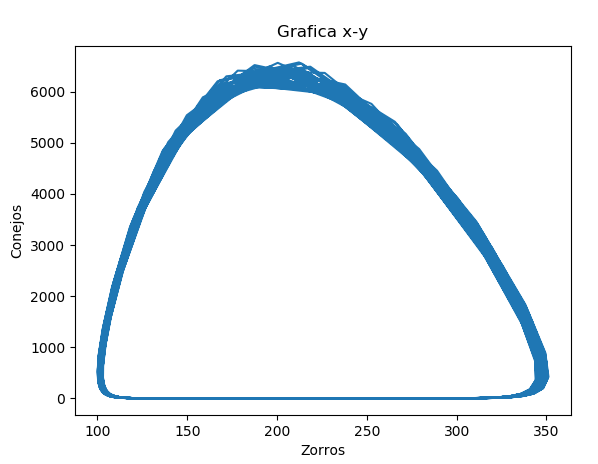
\includegraphics[width=0.5\textwidth]{screenshot011}}
	
\end{figure}

Este cambio nos da también unos resultados parecidos a los anteriores pero con dos pequeñas diferencias. La primera diferencia que se ve es que la poblacion de lobos no llega a bajar a niveles tan cercanos a 0 como en el caso anterior. Otro diferencia que se ve claramente es como el numero de conejos no da aumenta igualmente en todos los picos de crecida. Se observa una pequeña bajada a lo largo del tiempo en el máximo de conejos que vamos alcanzando, esto también se ve en el grafico que mostramos los conejos y los zorros en proporción, quedando la linea superior mucho mas ancha, al cambiar los picos máximos en cada ejecucion. 
\newpage

Como pequeña curiosidad vamos a probar aumentando el tiempo final para ver si esto se cumple y los valores de los conejos sigue disminuyendo. He realizado un ejecución con un tiempo de final de 200000.
\begin{figure}[H]
	\centering
	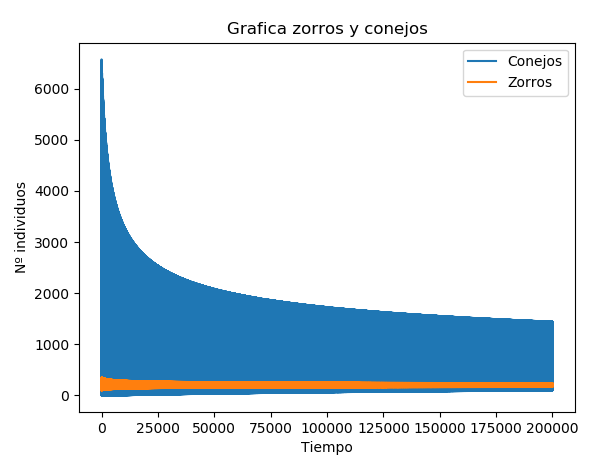
\includegraphics[width=1\linewidth]{screenshot012}
	\caption{}
\end{figure}
En la grafica se ve claramente como el numero de conejos se va reduciendo y también se ve como el numero de zorros toma valores mas centrales y alejándose mas del 0 y de los picos mas altos del principio. Esto se puede dar estabilizarse la poblacion en niveles mas centrales de forma mas rápida no dejando llegar a la otra poblacion a un extremo mayor. Por ejemplo si la poblacion de zorros aumentara mas rápido por cada ejecucion, alcanzaría antes un nivel en el que fueran los suficientes zorros para hacer disminuir la población de conejos, llegando un punto en el que ya no puede aumentar mas rápido y quedándose las poblaciones de zorros y conejos en estos niveles, sin aumentar ni bajar los valores máximos y mínimos. Se ve como los zorros aumentan y se van alejando de los valores mas bajos, lo que podría dar a entender que ocurre lo explicado anteriormente.
\newpage

\subsubsection{Aumento de la importancia de la comida}
En este caso se aumentara $a_{21}$ cambiando el valor de 0.0004 a 0.0006. Vamos a mostrar las graficas para poder analizarlas. 
\begin{figure}[H]
	\centering
	\subfloat{
		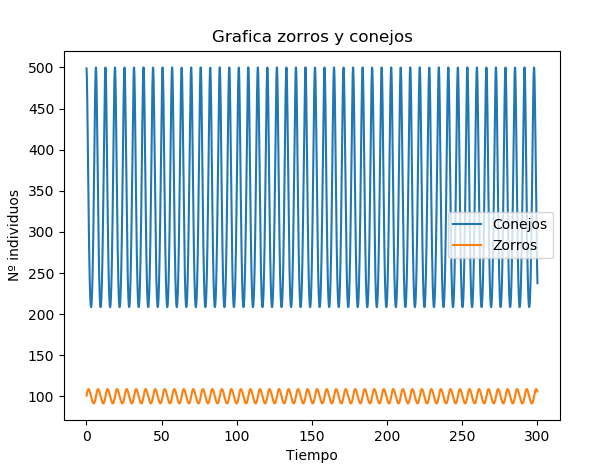
\includegraphics[width=0.5\textwidth]{screenshot014}}
	\subfloat{
		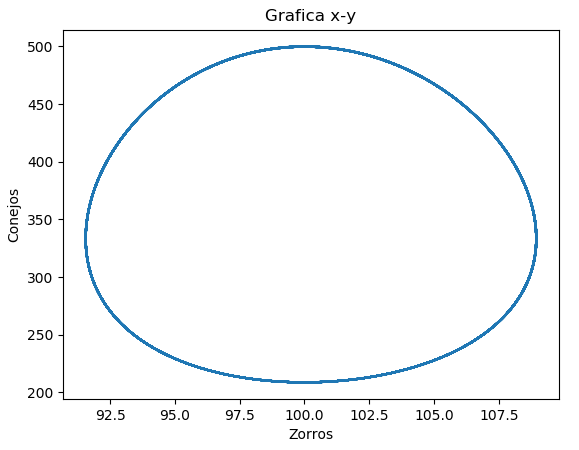
\includegraphics[width=0.5\textwidth]{screenshot013}}
	
\end{figure}

En este caso se ve como la población se estabiliza y conseguimos algo parecido al caso en el que se aumenta los conejos, aunque en este caso los valores máximos y mínimos son algo mayores. También se nota en la grafica que representamos los dos valores, donde el circulo esta un poco mas achatado que el anterior debido a esto.
\newline

Al aumentar la importancia de una comida, hacemos que los zorros necesiten cazar menos para estar bien nutridos y esto hace que aunque no aumentemos el numero de conejos al necesitar menos la población se estabilice y no se acerque a la extinción.

\subsubsection{Aumento de la mortalidad de los zorros.}
Para este cambio aumentaremos el paramento $a_{22}$, cambiándolo de 0.2 a 0.3, esto hace que se doble la mortalidad de los zorros y se acorte su vida máxima. Vamos a ver como afecta esto a nuestras graficas.

\begin{figure}[H]
	\centering
	\subfloat{
		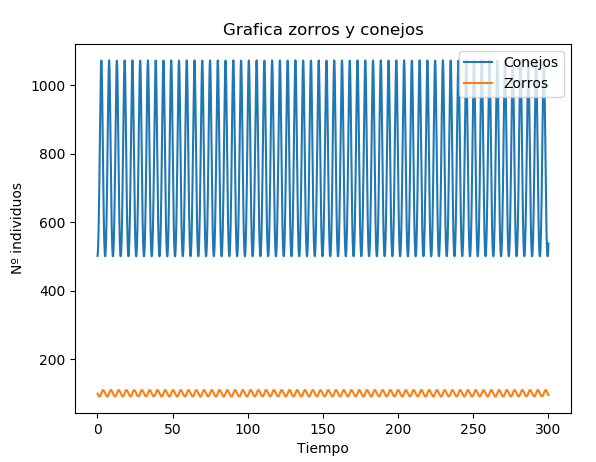
\includegraphics[width=0.5\textwidth]{screenshot016}}
	\subfloat{
		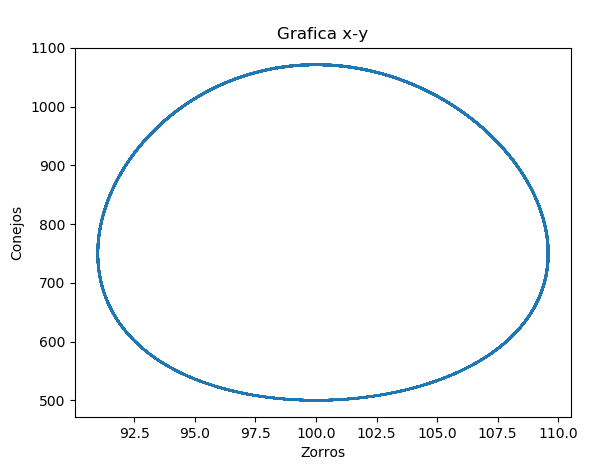
\includegraphics[width=0.5\textwidth]{screenshot015}}
	
\end{figure}

En este caso también obtenemos una población equilibrada para ambas especies. Esto se debe a lo explicado anteriormente. Como los zorros en este caso mueren mas rápido al tener una vida menos lagar, tendremos menos zorros para cazar y la poblacion se estabiliza sin la necesidad de aumentar los conejos. En este caso los picos máximos y mínimos son algo mayores aunque se podrían recortar un poquito mas y aproximarlos al ejemplo anterior cambiando por ejemplo $a_{22}$ a un valor algo mas bajo que 0.3 y mayor que 0.2, como podría ser 0.25.

\subsection{Comprar Euler y Runge-Kutta}
Para esto vamos a utilizar los valores por defecto en todos los parámetros excepto en la población de conejos que la aumentaremos a 600 para que tengamos una variación en las poblaciones.

A continuación mostraremos las graficas con Euler seguidas a continuación de las graficas con Runge-Kuta:
\begin{enumerate}
	\item \textbf{Euler:} 
	\begin{figure}[H]
		\centering
		\subfloat{
			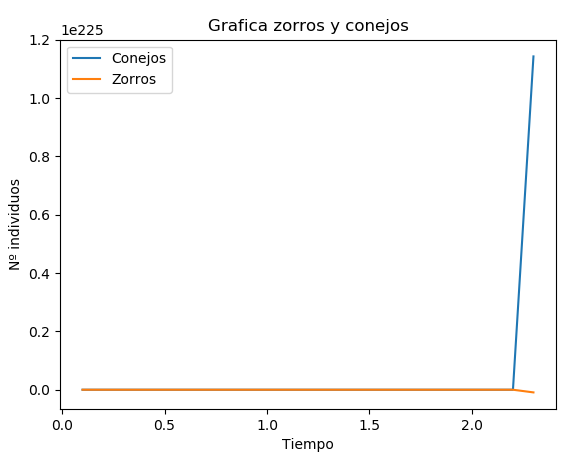
\includegraphics[width=0.5\textwidth]{screenshot017}}
		\subfloat{
			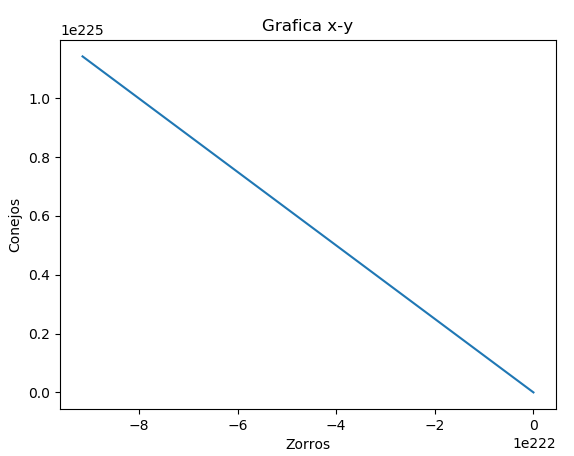
\includegraphics[width=0.5\textwidth]{screenshot018}}
		
	\end{figure}
	\begin{figure}
		\centering
		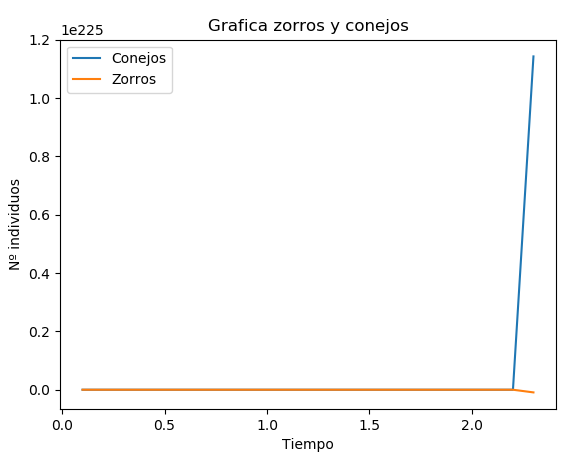
\includegraphics[width=0.7\linewidth]{screenshot017}
		\caption{}
		\label{fig:screenshot017}
	\end{figure}
	\begin{figure}
		\centering
		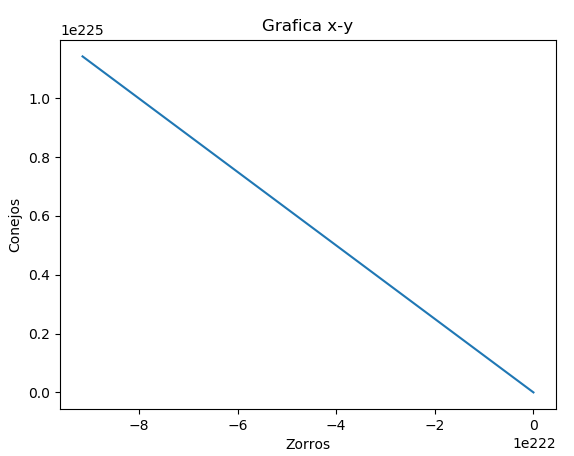
\includegraphics[width=0.7\linewidth]{screenshot018}
		\caption{}
		\label{fig:screenshot018}
	\end{figure}
	
	\item \textbf{Runge-Kuta:} 
	\begin{figure}[H]
		\centering
		\subfloat{
			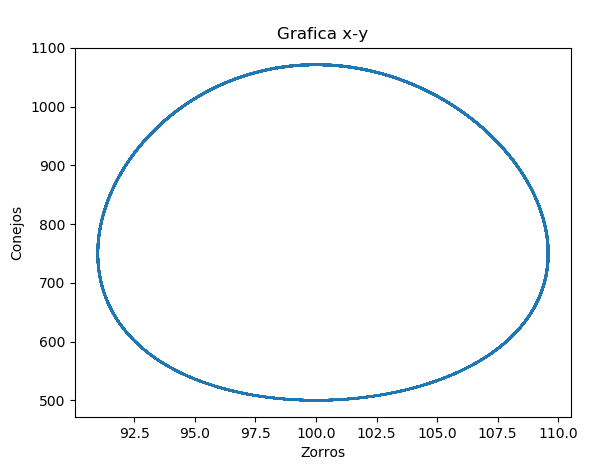
\includegraphics[width=0.5\textwidth]{screenshot015}}
		\subfloat{
			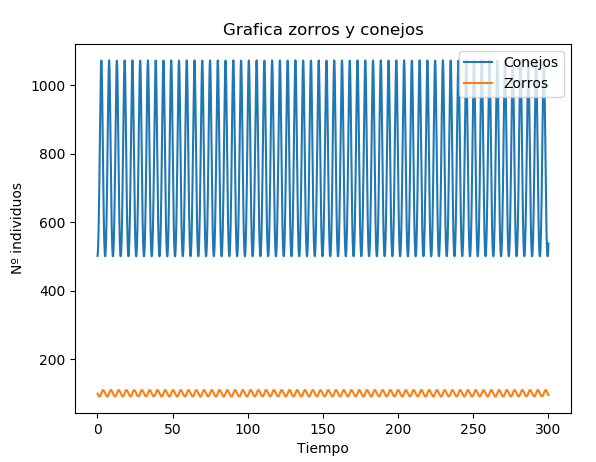
\includegraphics[width=0.5\textwidth]{screenshot016}}
		
	\end{figure}
	\begin{figure}[H]
		\centering
		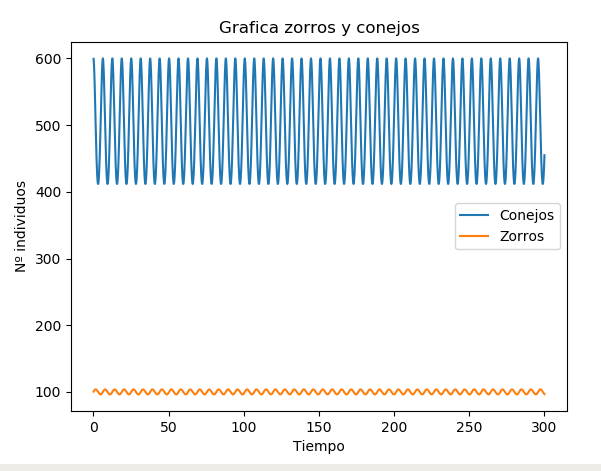
\includegraphics[width=1\linewidth]{screenshot005}
		\caption{}
		\label{fig:screenshot005}
	\end{figure}
	\begin{figure}[H]
		\centering
		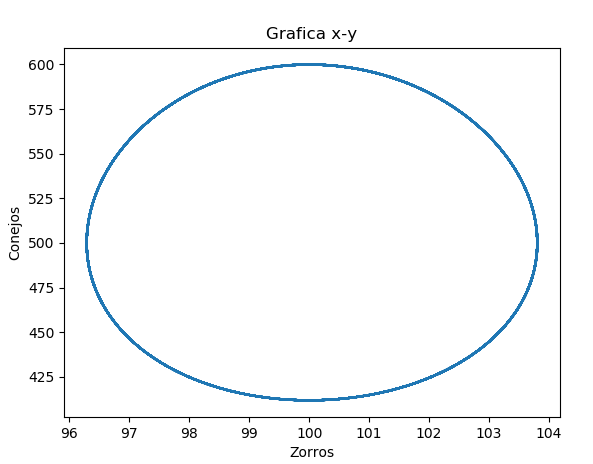
\includegraphics[width=1\linewidth]{screenshot006}
		
	\end{figure}
	
\end{enumerate}



\end{document}







